\chapter{Apéndice}
En este apartado se introduce la documentación de la biblioteca,
con la descripción de cada clase. El objetivo de dicha documentación es 
facilitar al usuario final el uso de la biblioteca, la cual puede 
consultar online, para tener una referencia y breve
descripción de los métodos.

Aquí se introduce la versión pdf de dicha documentación pero
podemos encontrar dicha documentación en línea en el repositorio
del proyecto en GitHub \cite{Miki97TFGOutlierDetectionHttps} y en el repositorio de 
PyPI \cite{PyDBODDistancesBased}


\setboolean{@twoside}{false}


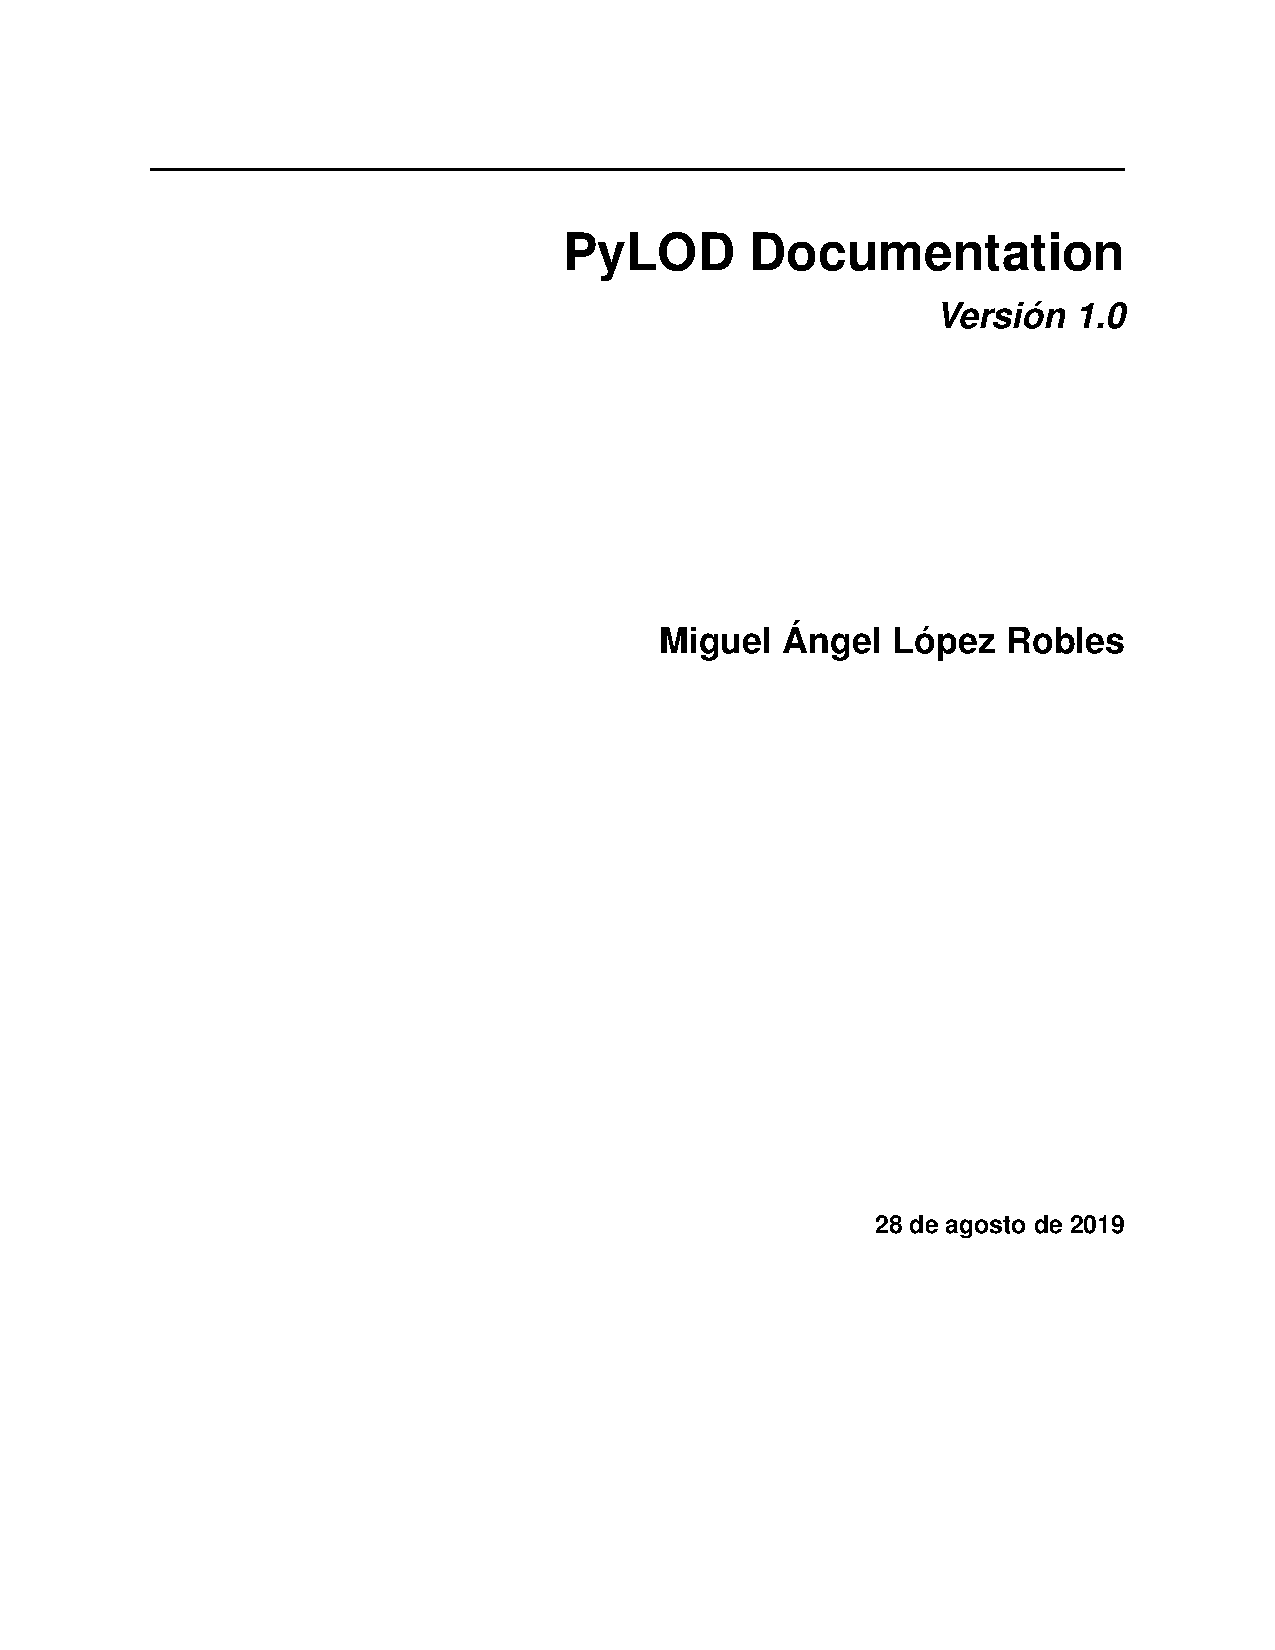
\includepdf[scale= 1,pages=-, ]{documentation.pdf}
%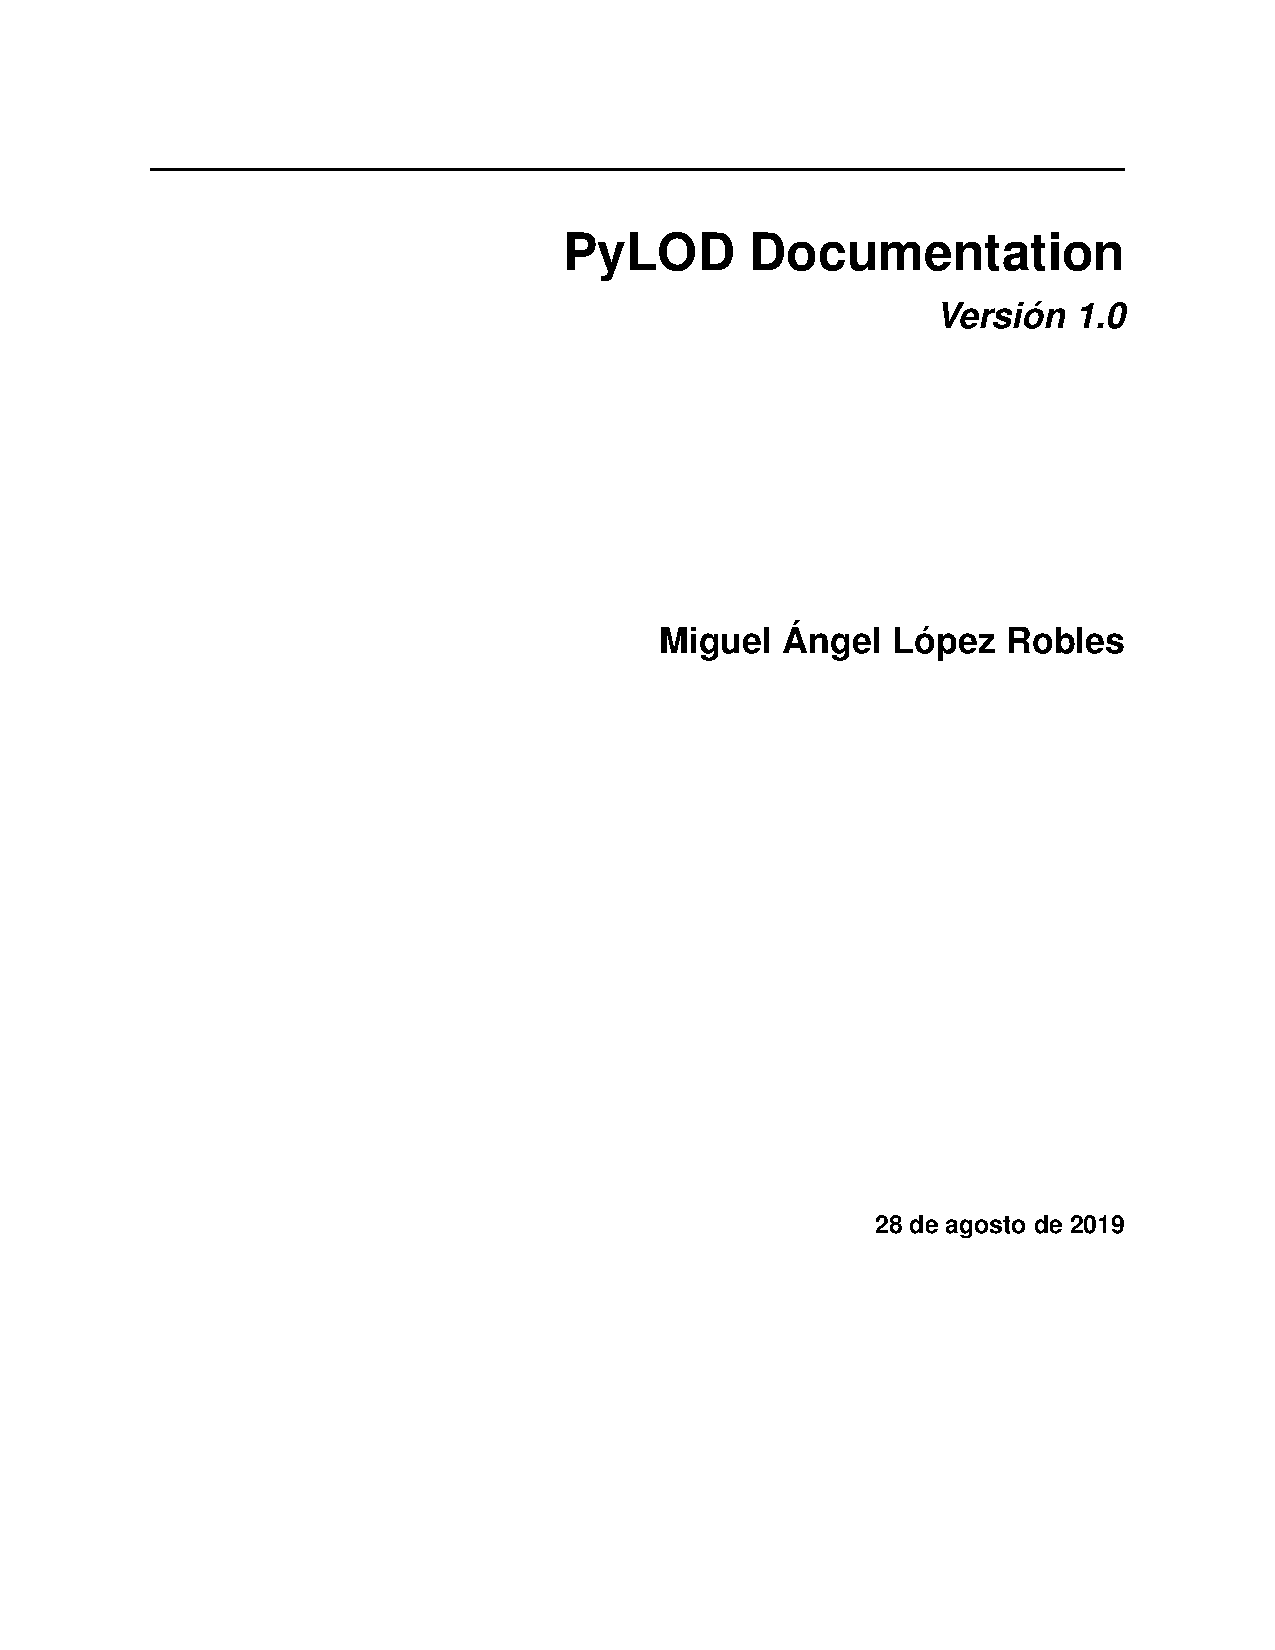
\includepdf[scale=0.8,pages=-,pagecommand=\subsection{blub}]{documentation}